\documentclass[conference]{IEEEtran}

% ----------------------------------------------------------------
% Packages
% ----------------------------------------------------------------
\usepackage{cite}
\usepackage{amsmath,amssymb,amsfonts}
\usepackage{booktabs}
\usepackage{array}
\usepackage{url}
\usepackage{microtype}
\usepackage{tikz}
\usetikzlibrary{shapes.geometric,arrows.meta,positioning,fit}

% ----------------------------------------------------------------
% Title, Author
% ----------------------------------------------------------------
\title{Improved Priority Exchange Server}

\author{%
  \IEEEauthorblockN{Sumon Boiddo}
  \IEEEauthorblockA{%
    BEng Electronic Engineering, Group~B, Team~6\\
    Hochschule Hamm-Lippstadt (HSHL), Lippstadt, Germany\\
    Matriculation Number:~2220054\\
    sumon.boiddo@stud.hshl.de}
}

\begin{document}

\maketitle

% ----------------------------------------------------------------
\begin{abstract}
This paper presents a comprehensive analysis of the Improved
Priority Exchange (IPE) server, an Earliest Deadline First
(EDF)-based aperiodic server designed for hard real-time systems.
IPE achieves near-optimal aperiodic responsiveness by
precomputing the idle-time profile of the optimal Earliest
Deadline Late (EDL) server offline and replaying it at runtime
through the priority-exchange mechanism of the Dynamic Priority
Exchange (DPE) server. This approach avoids EDL's prohibitive
runtime recomputation cost while delivering nearly identical
aperiodic response times. The paper covers the formal model,
the replenishment and exchange algorithm, the schedulability
condition, a structured comparison with neighbouring aperiodic
servers (PE, DPE, EDL, TBS), a critical evaluation of
strengths and limitations, a scalability analysis, and a
discussion of suitable and unsuitable embedded systems
application scenarios. Proposed extensions address memory
reduction, multi-core deployment, and dynamic adaptability.
The primary reference is Buttazzo, \emph{Hard Real-Time
Computing Systems}~\cite{buttazzo2011}, Chapter~6.
\end{abstract}

\begin{IEEEkeywords}
real-time systems, aperiodic server, EDF scheduling,
priority exchange, IPE, embedded systems
\end{IEEEkeywords}

% ================================================================
\section{Introduction}
% ================================================================

Hard real-time embedded systems must simultaneously satisfy two
conflicting demands. Periodic tasks execute at fixed, predictable
intervals and carry hard deadlines whose violation constitutes
system failure. Aperiodic tasks arrive unpredictably and must
be served as quickly as possible, yet their service must never
jeopardise periodic deadlines. Naive solutions perform poorly:
background execution makes aperiodic response times
unacceptably long under load, while running aperiodic requests
at the highest fixed priority risks causing periodic deadline
misses~\cite{buttazzo2011}.

A family of \emph{aperiodic servers} has been developed to
resolve this tension. Each server reserves a portion of the
processor for aperiodic service while guaranteeing all periodic
deadlines. Servers differ in the scheduling algorithm used for
periodic tasks, the mechanism by which server capacity is
maintained, and the responsiveness achieved for aperiodic
requests.

The Improved Priority Exchange (IPE) server~\cite{spuri1996}
occupies a distinctive position in this design space. It
combines the dynamic-priority (EDF) scheduling framework of
the DPE server with the precomputed idle-time profile of the
optimal EDL server, reaching near-optimal responsiveness at a
practical runtime cost. This paper synthesises a technical
understanding of IPE (Section~\ref{sec:technical}), places it
in its scientific context (Section~\ref{sec:context}), and
critically evaluates its strengths, limitations, scalability,
and applicability (Sections~\ref{sec:critical}--\ref{sec:extensions}).
AI usage is documented per the protocol submitted alongside
this milestone~\cite{ai_protocol_m4}.

% ================================================================
\section{Technical Background: The IPE Server}
\label{sec:technical}
% ================================================================

\subsection{Problem Setting}

A real-time system runs $n$ periodic tasks
$\tau_1,\ldots,\tau_n$, each characterised by a period~$T_i$,
a worst-case execution time~$C_i$, and an implicit deadline
$D_i = T_i$. All tasks are activated simultaneously at
$t = 0$. The total periodic utilisation is
$U_p = \sum_{i=1}^{n} C_i/T_i$. Under EDF the system is
schedulable as long as $U_p \leq 1$, making up to $100\%$ of
the processor available, compared with approximately $69\%$
under Rate Monotonic (RM) for large task
sets~\cite{buttazzo2011}. This larger utilisation bound is the
primary reason for choosing EDF as the scheduling algorithm
for an aperiodic server.

Alongside the periodic tasks the system receives aperiodic
requests at random times with soft (non-hard) deadlines. The
challenge is to serve these requests quickly without
endangering any periodic deadline.

\subsection{Motivation: EDL, DPE, and the Role of IPE}

Two EDF-based aperiodic servers existed before IPE was
proposed:
\begin{itemize}
  \item The \emph{Earliest Deadline Late (EDL)}
    server~\cite{spuri1994} is provably optimal---it achieves
    the minimum possible aperiodic waiting time among all
    scheduling strategies~\cite{chetto1989}. However, EDL
    recomputes the full idle-time schedule at each aperiodic
    arrival, incurring prohibitive runtime cost that makes it
    impractical for deployment.
  \item The \emph{Dynamic Priority Exchange (DPE)}
    server~\cite{spuri1996} avoids wasting free processor time
    by lending its capacity to periodic tasks and saving an
    equal amount for later reuse. Its replenishment strategy
    does not, however, exploit the EDL idle-time structure,
    so it falls noticeably short of optimality.
\end{itemize}

IPE's core contribution is conceptually simple: the idle-time
pattern of the EDL schedule is deterministic and repeats
every hyperperiod $H = \operatorname{lcm}(T_1,\ldots,T_n)$.
This pattern can therefore be computed \emph{once, offline},
before the system starts, and stored in compact arrays. At
runtime IPE replays these precomputed values through the DPE
mechanism, achieving near-optimal responsiveness without
EDL's runtime cost~\cite{buttazzo2011}.

Figure~\ref{fig:lineage} illustrates the design lineage from
PE through DPE to IPE.

% --- Lineage figure -------------------------------------------
\begin{figure}[t]
\centering
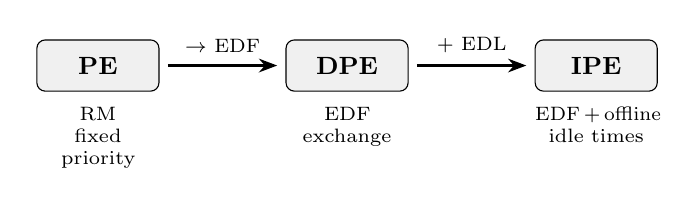
\begin{tikzpicture}[
  server/.style={rectangle, draw, rounded corners=3pt,
    font=\small\bfseries, minimum width=1.55cm,
    minimum height=0.65cm, fill=gray!12},
  desc/.style={font=\scriptsize, text width=1.55cm, align=center},
  arr/.style={-Stealth, thick, shorten >=3pt, shorten <=3pt},
  lbl/.style={font=\scriptsize, above, yshift=1pt}
]
  \node[server] (pe)  {PE};
  \node[desc, below=2pt of pe]  {RM\\fixed priority};
  \node[server, right=1.6cm of pe]  (dpe) {DPE};
  \node[desc, below=2pt of dpe] {EDF\\exchange};
  \node[server, right=1.6cm of dpe] (ipe) {IPE};
  \node[desc, below=2pt of ipe] {EDF\,+\,offline\\idle times};
  \draw[arr] (pe)  -- node[lbl]{$\to$ EDF} (dpe);
  \draw[arr] (dpe) -- node[lbl]{$+$ EDL} (ipe);
\end{tikzpicture}
\caption{Design lineage of the IPE server. PE introduced
  the priority-exchange idea under RM; DPE moved it to EDF;
  IPE added the precomputed EDL idle-time
  profile~\cite{spuri1996}.}
\label{fig:lineage}
\end{figure}
% --------------------------------------------------------------

\subsection{Formal Model}

The availability function $\omega(t)$ describes processor
idleness:
\begin{equation}
  \omega(t) =
  \begin{cases}
    1 & \text{if the CPU is idle at time } t,\\
    0 & \text{if the CPU is busy at time } t.
  \end{cases}
\end{equation}
The total idle time in an interval $[t_1,t_2]$ is:
\begin{equation}
  \Omega(t_1,t_2) = \int_{t_1}^{t_2} \omega(t)\,\mathrm{d}t.
\end{equation}

Among all EDF strategies, EDL maximises $\Omega(0,t)$ for
every $t$, meaning it releases processor time as early as
possible~\cite{chetto1989}. Because free time comes earlier,
arriving aperiodic requests are served sooner. IPE
precomputes this EDL idle-time profile for one hyperperiod
and stores it in two arrays:
\begin{itemize}
  \item $E = (e_0, e_1, \ldots, e_p)$: the start times of
    idle intervals within one hyperperiod;
  \item $D = (\Delta_0, \Delta_1, \ldots, \Delta_p)$: the
    corresponding durations of those intervals.
\end{itemize}

The IPE server is then defined by the following
rules~\cite{spuri1996}:
\begin{enumerate}
  \item The server starts with capacity~$0$.
  \item At each time instant $t = e_i + kH$
    ($k = 0,1,2,\ldots$), server capacity is replenished
    by $\Delta_i$ units.
  \item The server always runs at the highest priority
    in the system.
  \item All remaining rules---serving aperiodic requests,
    exchanging and saving capacity, and spare-time
    reclaiming---are inherited from the DPE server.
\end{enumerate}

\subsection{Schedulability Condition}

The periodic tasks together with the IPE server are
schedulable---no hard deadline is ever missed---if and only
if:
\begin{equation}
  U_p \leq 1.
  \label{eq:sched}
\end{equation}
The server automatically receives the remaining bandwidth
$1 - U_p$ for aperiodic service~\cite{spuri1996}. This is an
exact EDF condition, not a heuristic bound.

\subsection{Operating Algorithm}

Figure~\ref{fig:flowchart} shows the IPE operational cycle.
Four rules govern the server's behaviour at each scheduling
event:

\paragraph{Replenishment} At each precomputed instant
$t = e_i + kH$ the server capacity increases by $\Delta_i$
units, exactly mirroring the stored EDL idle time.

\paragraph{Exchange} When capacity is available but no
aperiodic request is waiting, the capacity is exchanged: a
periodic task executes immediately, and an equal amount of
capacity is saved for future use. No CPU time is wasted.

\paragraph{Consumption} When an aperiodic request arrives
and capacity is positive, the request executes immediately at
the highest priority, consuming capacity at a one-to-one
rate. When capacity reaches zero, aperiodic service is
suspended until the next replenishment.

\paragraph{Spare-time reclaiming} If a periodic task
finishes before its worst-case execution time, the remaining
slack is added to the server's capacity. This is safe because
the time was already reserved for the periodic task and
imposes no additional load~\cite{buttazzo2011}.

% --- Operational flowchart ------------------------------------
\begin{figure}[t]
\centering
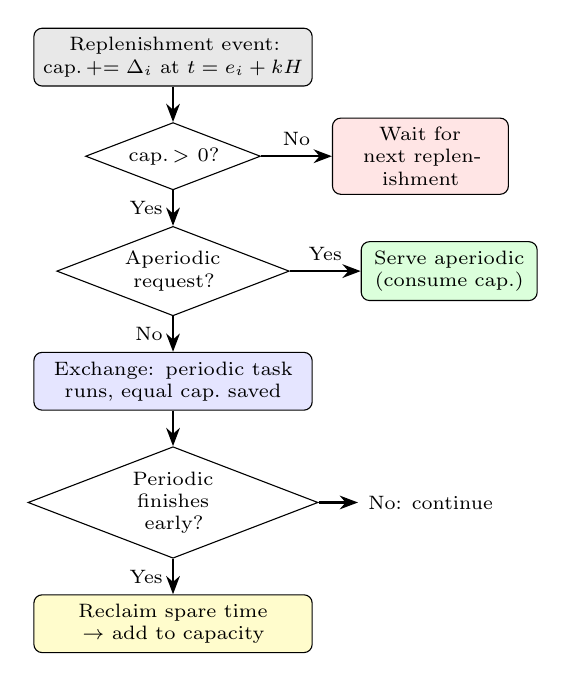
\begin{tikzpicture}[
  node distance=0.38cm and 0.5cm,
  box/.style={rectangle, draw, rounded corners=3pt,
    font=\scriptsize, text width=3.3cm, align=center,
    minimum height=0.6cm},
  dec/.style={diamond, draw, font=\scriptsize,
    text width=1.4cm, align=center, aspect=2.6,
    inner sep=1pt},
  arr/.style={-Stealth, thick},
  lbl/.style={font=\scriptsize}
]
  \node[box, fill=gray!18] (rep)
    {Replenishment event:\\cap.\,$\mathrel{+}= \Delta_i$
      at $t = e_i + kH$};
  \node[dec, below=0.45cm of rep] (cap)
    {cap.\,$> 0$?};
  \node[dec, below=0.45cm of cap] (req)
    {Aperiodic\\request?};
  \node[box, right=0.9cm of cap, fill=red!10, text width=2.0cm]
    (wait) {Wait for\\next replenishment};
  \node[box, below=0.45cm of req, fill=blue!10] (exc)
    {Exchange: periodic task\\runs, equal cap.\ saved};
  \node[box, right=0.9cm of req, fill=green!14, text width=2.0cm]
    (srv) {Serve aperiodic\\(consume cap.)};
  \node[dec, below=0.45cm of exc] (spr)
    {Periodic\\finishes early?};
  \node[box, below=0.45cm of spr, fill=yellow!20] (rcl)
    {Reclaim spare time\\$\to$ add to capacity};

  \draw[arr] (rep) -- (cap);
  \draw[arr] (cap) -- node[lbl,left]{\scriptsize Yes} (req);
  \draw[arr] (cap) -- node[lbl,above]{\scriptsize No}  (wait);
  \draw[arr] (req) -- node[lbl,left]{\scriptsize No}   (exc);
  \draw[arr] (req) -- node[lbl,above]{\scriptsize Yes} (srv);
  \draw[arr] (exc) -- (spr);
  \draw[arr] (spr) -- node[lbl,left]{\scriptsize Yes}  (rcl);
  \draw[arr] (spr.east) -- ++(0.5,0)
    node[right,font=\scriptsize]{No: continue};
\end{tikzpicture}
\caption{IPE server operational cycle. At each replenishment
  the server decides whether to serve an aperiodic request,
  exchange capacity with a periodic task, or wait. Spare
  time from early-finishing periodic tasks is
  reclaimed~\cite{buttazzo2011}.}
\label{fig:flowchart}
\end{figure}
% --------------------------------------------------------------

% ================================================================
\section{Scientific Context: Related Approaches}
\label{sec:context}
% ================================================================

\subsection{The Aperiodic Server Landscape}

Aperiodic servers belong to two families according to the
scheduling algorithm used for periodic tasks~\cite{buttazzo2011}.
The \emph{fixed-priority} (RM) family includes the Polling
Server (PS), the Deferrable Server (DS), the Priority Exchange
(PE) server, and the Sporadic Server (SS). The
\emph{dynamic-priority} (EDF) family includes the Dynamic
Priority Exchange (DPE) server, the Dynamic Sporadic Server
(DSS), the Total Bandwidth Server (TBS), the Earliest Deadline
Late (EDL) server, and IPE itself.

IPE occupies the end of a clear design lineage: the PE
server was extended to EDF as DPE, and DPE was then improved
into IPE by grafting in the precomputed EDL idle-time
structure~\cite{spuri1996}.

\subsection{Structured Comparison}

Table~\ref{tab:comparison} compares IPE with its four nearest
neighbours across the scheduling algorithm used, the aperiodic
responsiveness achieved, and the principal limitation.

\begin{table}[t]
\caption{Comparison of Aperiodic Server Approaches}
\label{tab:comparison}
\centering
\renewcommand{\arraystretch}{1.25}
\begin{tabular}{@{}p{1.2cm}p{0.75cm}p{1.35cm}p{2.5cm}@{}}
\toprule
\textbf{Server} & \textbf{Sched.} & \textbf{Resp.} &
  \textbf{Main limitation}\\
\midrule
PE   & RM  & Moderate    & Fixed priority; less responsive\\
DPE  & EDF & Good        & Periodic replenishment; not optimal\\
EDL  & EDF & Optimal     & Heavy runtime recomputation\\
TBS  & EDF & Very good   & No idle-time exploitation\\
IPE  & EDF & Near-optimal& High memory (non-harmonic periods)\\
\bottomrule
\end{tabular}
\end{table}

\paragraph{IPE vs.\ PE} PE is IPE's fixed-priority ancestor.
Moving the exchange idea to EDF and adding the precomputed
EDL idle times delivers substantially faster aperiodic
service~\cite{spuri1996}.

\paragraph{IPE vs.\ DPE} Both servers share the EDF scheduler
and the priority-exchange mechanism. The improvement in IPE
lies entirely in the replenishment policy: DPE uses a periodic
refill, whereas IPE replenishes at exactly the EDL idle-time
instants stored in the $E$ and $D$ arrays and always runs at
the highest priority~\cite{spuri1996}.

\paragraph{IPE vs.\ EDL} EDL is provably optimal~\cite{spuri1994}:
no scheduling strategy can reduce aperiodic waiting times
further. IPE comes extremely close to this bound but falls
marginally short in rare cases. The decisive advantage is
that IPE's heavy computation is performed offline, whereas
EDL recomputes at every aperiodic arrival. IPE therefore
trades a negligible margin of optimality for a dramatically
lower runtime cost, paying the difference in
memory~\cite{buttazzo2011}.

\paragraph{IPE vs.\ TBS} TBS assigns each aperiodic request
a deadline and schedules it directly under EDF with negligible
overhead and no stored tables~\cite{buttazzo2011}. It is
simpler and lighter than IPE but does not exploit the EDL
idle-time structure. Under heavy aperiodic load, IPE's
near-optimal responsiveness is noticeably better than TBS, at
the cost of offline precomputation and the memory required
for the $E$ and $D$ arrays.

\subsection{Engineering Trade-offs}

Four trade-offs characterise IPE's design position:

\textit{Optimality vs.\ practicality.} EDL is theoretically
optimal but practically infeasible due to runtime cost.
IPE sacrifices a small margin of optimality to become
deployable, performing the heavy work once at design time.

\textit{Runtime cost vs.\ memory cost.} Precomputing the
idle-time schedule shifts computation from runtime to the
offline phase. The benefit is low runtime overhead; the cost
is the memory required for the $E$ and $D$ arrays, which
grows with the hyperperiod $H$.

\textit{Performance vs.\ flexibility.} Because IPE is
tailored to a fixed, fully-known periodic task set, it cannot
accommodate a changing task set at runtime. Static high
performance is purchased at the expense of dynamic
adaptability.

\textit{Near-optimal performance vs.\ simplicity.} Compared
with TBS, IPE is more responsive but considerably more
complex to implement and deploy, requiring both the offline
precomputation step and the priority-exchange bookkeeping.

% ================================================================
\section{Critical Evaluation}
\label{sec:critical}
% ================================================================

\subsection{Concrete Strengths}

IPE's foremost strength is \emph{near-optimal aperiodic
responsiveness}. By replaying the precomputed EDL idle-time
profile, IPE serves aperiodic requests almost as fast as the
optimal EDL server and always at the highest system priority
when capacity is available~\cite{buttazzo2011}. At the same
time, its \emph{runtime overhead is low}: the work at each
scheduling event consists only of a capacity update and a
table lookup, comparable in cost to DPE~\cite{spuri1996}.

The \emph{priority-exchange mechanism} ensures no CPU time is
wasted: when no aperiodic request is pending, the server lends
its capacity to periodic tasks and saves an equal amount for
future use, and spare-time reclaiming further increases
effective processor utilisation. Finally, IPE provides a
\emph{formal, exact schedulability guarantee} under EDF
(equation~\eqref{eq:sched}), not a heuristic
bound~\cite{spuri1996}.

\subsection{Concrete Limitations and Risks}

IPE's main weakness is \emph{high memory cost}. The arrays
$E$ and $D$ must cover one full hyperperiod
$H = \operatorname{lcm}(T_1,\ldots,T_n)$. When task periods
are non-harmonic, $H$ can grow exponentially with the number
of tasks, making the tables impractically
large~\cite{buttazzo2011}. This is IPE's principal
scalability bottleneck and the most significant obstacle to
deployment on memory-constrained embedded devices.

A second major limitation is the \emph{requirement for a
static task set}. IPE presupposes that all periodic task
parameters are known at design time and remain fixed
throughout operation. Any runtime modification to the task
set invalidates the precomputed arrays and removes all
schedulability guarantees.

Additional limitations include the \emph{need for an
EDF-capable operating system} (excluding fixed-priority
platforms such as AUTOSAR-based systems),
\emph{implementation complexity} relative to simpler servers
such as TBS, and the fact that IPE is not \emph{fully}
optimal---the EDL server can be marginally better in rare
cases~\cite{spuri1996}.

\subsection{Hidden and Potentially Unrealistic Assumptions}

Several assumptions underlying the basic IPE model deserve
scrutiny in practical deployments:

\begin{itemize}
  \item \textit{Accurate WCET estimates.} IPE assumes each
    periodic task's worst-case execution time is known
    exactly. In practice WCET is hard to bound tightly, and
    overestimates lead to unnecessary capacity reservation
    while underestimates can cause deadline misses.
  \item \textit{Full preemptibility.} The model assumes any
    task can be preempted instantly. Real systems contain
    non-preemptible critical sections, interrupt handlers,
    and device-driver code that introduce blocking delays not
    captured by the basic model.
  \item \textit{Implicit deadlines and synchronous release.}
    IPE assumes $D_i = T_i$ and simultaneous task activation
    at $t = 0$. Systems with constrained or arbitrary
    deadlines, or staggered phase offsets, require extended
    analysis.
  \item \textit{Single processor.} The model is defined
    exclusively for one CPU. Modern embedded systems are
    commonly multi-core, and the basic IPE formulation does
    not extend to them.
\end{itemize}

% ================================================================
\section{Scalability Analysis}
\label{sec:scalability}
% ================================================================

IPE scales well in \emph{time} but poorly in \emph{memory}.
At runtime the server's activity per scheduling event is
bounded and independent of the number of tasks: it consists
of a table lookup, a capacity update, and optionally a
spare-time reclaim. The offline computation of the $E$ and
$D$ arrays grows with the hyperperiod but is a one-time
design-time cost that does not affect runtime performance.

Memory, by contrast, scales with the hyperperiod. For
harmonically-related periods the hyperperiod equals the
largest period, so the tables remain small. For non-harmonic
periods the hyperperiod is the least common multiple of all
task periods, which can grow by orders of magnitude with each
additional task, making IPE impractical on memory-constrained
devices. Memory is therefore IPE's hard scalability limit.

Overall, IPE is best suited to systems with a small number
of harmonically-related tasks and does not scale to large or
non-harmonic task sets on limited-memory hardware.

% ================================================================
\section{Application Discussion}
\label{sec:applications}
% ================================================================

\subsection{Suitable Scenario: Robot Motor Controller}

A robot motor controller is a strong match for IPE. Its fixed
control loops---for example sensor reading at 1~kHz and
actuator update at 500~Hz---are harmonically related, known at
design time, and carry hard deadlines. Alongside these, the
controller receives soft aperiodic events such as operator
commands, status queries, and diagnostic messages.

IPE fits this scenario because the periodic task set is
static and fully known (enabling offline precomputation of
the $E$ and $D$ arrays); the harmonic periods keep the
hyperperiod small (keeping the tables compact); the
controller runs on a single processor under an EDF scheduler;
and IPE guarantees all hard control deadlines while serving
aperiodic commands with near-optimal speed.

\subsection{Unsuitable Scenario: AUTOSAR-Based ECU}

An automotive engine-control unit (ECU) running an
AUTOSAR-based real-time operating system illustrates where
IPE fails. AUTOSAR mandates fixed-priority scheduling
(RM-style), providing no EDF scheduler and therefore no
platform on which IPE can run. Additionally, AUTOSAR ECUs
frequently modify their active task sets at runtime through
mode switches and optional function-block activation, which
would immediately invalidate IPE's precomputed arrays.

On such a platform, fixed-priority aperiodic servers---the
Polling Server, the Deferrable Server, or the Sporadic
Server---are the appropriate choice. More generally, IPE is
unsuitable for any system with a dynamic task set, a
non-EDF scheduler, non-harmonic periods on a
memory-limited device, or a multi-core processor.

% ================================================================
\section{Open Questions and Proposed Extensions}
\label{sec:extensions}
% ================================================================

The limitations identified above motivate several directions
for future work. These are proposed extensions based on the
analysis in this paper and are not claims about existing
published solutions.

\begin{itemize}
  \item \textit{Reduced-memory IPE.} Approximate or compress
    the $E$ and $D$ arrays to make IPE deployable on systems
    with non-harmonic periods and limited memory, while
    quantifying the responsiveness penalty introduced by
    approximation. This directly addresses IPE's principal
    limitation.
  \item \textit{Multi-core IPE.} Extend the single-processor
    IPE model to multi-core architectures, where per-core
    servers must coordinate capacity exchange without
    excessive synchronisation overhead.
  \item \textit{Adaptive IPE.} Allow incremental online
    updates to the precomputed arrays when the task set
    changes at runtime, making IPE applicable to
    semi-dynamic systems without full offline recomputation.
  \item \textit{Robust IPE under WCET uncertainty.}
    Introduce a safety margin in the precomputed idle-time
    profile to tolerate imprecise WCET estimates and variable
    execution times while maintaining the schedulability
    guarantee.
\end{itemize}

An open theoretical question is whether a closed-form
worst-case response-time bound for aperiodic requests under
IPE can be derived, analogous to the response-time analysis
available for fixed-priority servers.

% ================================================================
\section{Conclusion}
% ================================================================

The Improved Priority Exchange server addresses a fundamental
challenge in hard real-time systems: how to serve
unpredictable aperiodic requests as quickly as possible
without endangering hard periodic deadlines. IPE achieves
this by combining two previously separate ideas---the
precomputed idle-time profile of the optimal EDL server and
the priority-exchange bookkeeping of the DPE server---into a
mechanism that is near-optimal in responsiveness and
practical in runtime cost.

IPE's strengths are its near-optimal aperiodic service, low
runtime overhead, CPU-efficient capacity management, and
exact formal schedulability guarantee. Its principal weakness
is memory consumption, which scales with the hyperperiod and
becomes prohibitive for non-harmonic task sets on
memory-constrained devices. Additional constraints---a static
task set, a single processor, and an EDF-capable
scheduler---limit its applicability to static embedded
systems with harmonic periods and sufficient memory.

Future work should focus on reducing the memory footprint,
extending the model to multi-core platforms, and enabling
online adaptation to changing task sets. These extensions
would broaden IPE's applicability while preserving its
central advantage of near-optimal aperiodic responsiveness
at practical runtime cost.

% ----------------------------------------------------------------
\begin{thebibliography}{9}

\bibitem{buttazzo2011}
G.\,C. Buttazzo,
\emph{Hard Real-Time Computing Systems: Predictable Scheduling
  Algorithms and Applications}, 3rd~ed.
Springer, 2011, ch.\,6 (Dynamic Priority Servers).

\bibitem{spuri1994}
M. Spuri and G. Buttazzo,
``Efficient Aperiodic Service under Earliest Deadline
  Scheduling,''
in \emph{Proc. IEEE Real-Time Systems Symposium (RTSS)}, 1994.

\bibitem{spuri1996}
M. Spuri and G. Buttazzo,
``Scheduling Aperiodic Tasks in Dynamic Priority Systems,''
\emph{Real-Time Systems}, vol.\,10, no.\,2, March 1996.

\bibitem{lehoczky1987}
J. Lehoczky, L. Sha, and J. Strosnider,
``Enhanced Aperiodic Responsiveness in Hard Real-Time
  Environments,''
in \emph{Proc. IEEE Real-Time Systems Symposium (RTSS)}, 1987.

\bibitem{chetto1989}
H. Chetto and M. Chetto,
``Some Results of the Earliest Deadline Scheduling
  Algorithm,''
\emph{IEEE Trans. Software Engineering}, vol.\,15, no.\,10,
1989.

\bibitem{ai_protocol_m4}
S. Boiddo,
``AI Usage Protocol, Milestone~4 (Final Seminar Paper):
  Improved Priority Exchange Server,''
HSHL, 2026. Protocol version~0.2; JSON, BibTeX, and Jupyter
Notebook files submitted with this milestone.

\end{thebibliography}

\end{document}
